\documentclass[10pt]{article}

\usepackage[left=3cm, right=3cm,top=2cm,bottom=2cm]{geometry}
\usepackage{tikz}
\usepackage{graphicx}
\usepackage{wrapfig}
\usetikzlibrary{shapes, arrows}


\font\myfont=cmr12 at 12pt
\setlength{\parindent}{8ex}

\newcommand\encircle[1]{\tikz[baseline=(X.base)] \node (X) [draw, shape=circle, inner sep=0] {\strut #1};}

\tikzstyle{block} = [draw, fill=red!20, rectangle,
minimum height=3em, minimum width=5em]
\tikzstyle{blockA} = [draw, fill=blue!20, rectangle,
minimum height=3em, minimum width=5em]
\tikzstyle{blockB} = [draw, fill=green!20, rectangle,
minimum height=3em, minimum width=5em]
\tikzstyle{sum} = [draw, fill=red!20, circle, node distance=2cm]
\tikzstyle{input} = [coordinate]
\tikzstyle{output} = [coordinate]
\tikzstyle{pinstyle} = [pin edge={-to,thin,black}]

\title{\bf{The Piano}}
\author{}
\author{\vspace{-2ex}}
\date{}
\date{\vspace{-2ex}}


\begin{document}


\begin{flushright}
    $_*$\underline{Group : 22}
\end{flushright}
\vspace{-10ex}
{\let\newpage\relax\maketitle}
\vspace{-12ex}
\section*{Introduction}
\vspace{-1.5ex}
Piano is one of the most pleasant musical instruments. It operates completely in a mechanical manner using vibration of differently tensed strings to produce musical notes. Our project idea is based on mimicking the operation using analog electronic components. Synthesizing signals with various frequencies and characteristics relevant to exact same notes which are produced by a real piano. This feasibility report will address the basic implementation strategies available in our analog design to generate a pleasant musical sound.
\vspace{-1ex}
\section*{Literature Review}
\vspace{-1.5ex}
Analog signal generator hidden inside the abstraction, is the starting point of most electronic circuits. Designs available in the market generate a variety of waveforms and frequency ranges according to the application. To generate a low-frequency sine-wave, available circuits engage a Wien bridge oscillator. This can be taken as the basic building block of piano since all tones can be visualized as the addition of different sine wave components. The concept of switching a connection with another circuit using a relay operation is common in analog design. This can be included in the piano design to mimic the action of the damping pedal.
\par
Old sound systems used an audio equalizer using RLC circuit to lower or boost certain frequency ranges specifically. This can be utilized in our piano to change the softness of the generated sound. In earlier days, most of the sound devices available in the market starting from simple analog radio up to studio speakers engaged voltage amplifiers to amplify the audio signal to a sustainable level. The circuit design of amplifiers also had the capability of removing dc offset which is a danger to the speaker.
\vspace{-1ex}
\section*{Block Diagram}
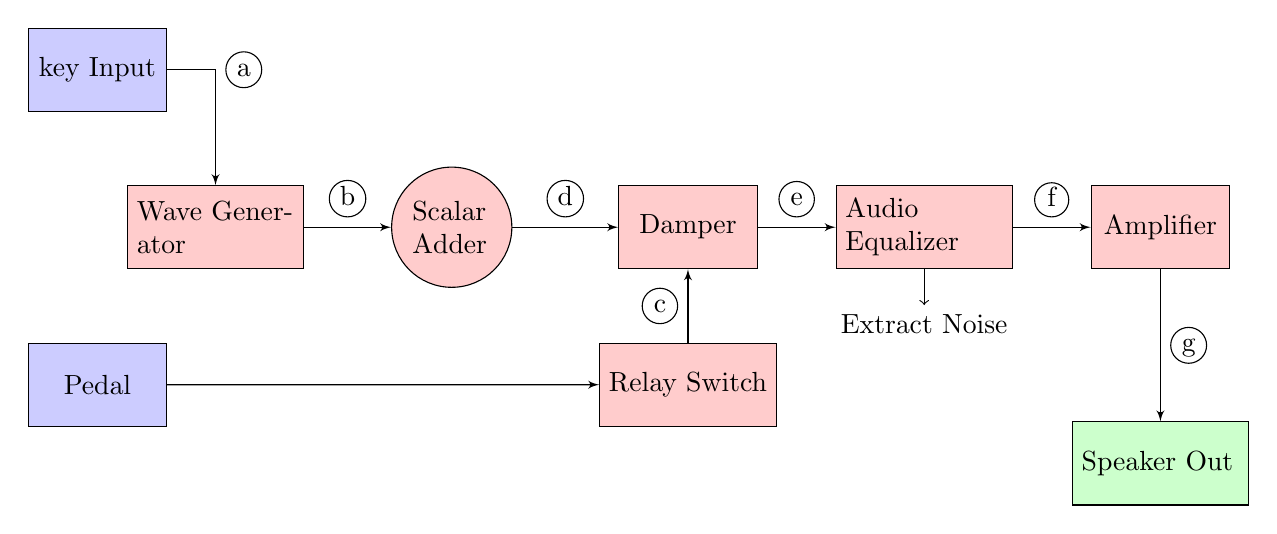
\begin{tikzpicture}[auto, node distance=3cm,>=latex']
    % We start by placing the blocks
    \node [blockA, name=keyInput] {key Input};
    \node [block, below of=keyInput,text width=2cm,yshift=1cm,xshift=1.5cm] (waveGenerator) {Wave Generator};
    \node[sum, right of =waveGenerator,text width=1cm,xshift=1cm](scalarAdder){Scalar Adder};
    \node[blockA, below of = keyInput,yshift=-1cm](pedal){Pedal};
    \node [block, right of = scalarAdder] (damper) {Damper};
    \node[block, below of = damper,yshift=1cm](switch){Relay Switch};
    \node [block, right of=damper,text width=2cm,, pin={[pinstyle]below:Extract Noise },node distance=3cm] (aE) {Audio Equalizer};
    \node[block, right of=aE](amplifier){Amplifier};
    \node[blockB,below of = amplifier,text width=2cm](speaker){Speaker Out};
    %\draw [->] (controller) -- node[name=u] {$u$} (system);
    %\node [output, right of=system] (output) {};


    % Once the nodes are placed, connecting them is easy. 
    \draw [draw,->] (keyInput.east) -| node {$\encircle{a}$} (waveGenerator.north);
    \draw [->] (waveGenerator) -- node {$\encircle{b}$} (scalarAdder);
    \draw[->](pedal) --node {} (switch);
    \draw[->](switch) --node {$\encircle{c}$} (damper);
    \draw[->](scalarAdder) --node {$\encircle{d}$} (damper);
    \draw[->](damper) --node {$\encircle{e}$} (aE);
    \draw[->](aE) --node {$\encircle{f}$} (amplifier);
    \draw[->](amplifier) --node {$\encircle{g}$} (speaker);
\end{tikzpicture}

\vspace{-8ex}
\section*{Analog Analysis}
\begin{itemize}
    \item[] $\encircle{a} : $ Analysing resistor values to be used in Wein-bridge that suit required frequency generation.
    \item[] $\encircle{b} : $ Pureness of sine waves generated with fundamental and over tone frequencies.
    \item[]  $\encircle{c} : $ Analysing the possiblity of switching and holding the damping operation.
    \item[] $\encircle{d} : $ Addition of the harmonic components according to the amplitude ratio.
    \item[] $\encircle{e} : $ Analyzation of exponential decay of audio signal.
    \item[] $\encircle{f} : $ Analyzing softness of sound by scaling different frequecy ranges.
    \item[] $\encircle{g} : $ Anlysing the output audio signal with different amplifiaction factor.
\end{itemize}


\section*{Methodology}

\subsubsection*{Analyzation of Piano Notes}
\vspace{-1.5ex}
Analyzing the frequency spectrum of sounds from each note of the piano, as to mimic the exact spectrum through the addition of sine waves.
\vspace{-1.5ex}
\subsubsection*{Wave Generation}
\vspace{-1.5ex}
We have decided to implement the Wein Bridge oscillator circuit to generate sine waves spans in the audio frequency range. The circuit allows modification of frequencies by interchanging values of resistance used. This character can be utilized to map the keys with corresponding wave generation.
\vspace{-1.5ex}
\subsubsection*{Damping of Audio Signals}
\vspace{-1.5ex}
As a step of mimicing the sound from Piano we need to decay the audio signal in an exponential manner. As of now, it is decided to implement some strategy to compensate the energy stored in wave inorder to get a decay in loudness with time.
\vspace{-1.5ex}
\subsubsection*{Amplification}
\vspace{-1.5ex}
As a step of getting audible sound from the piano, we decided to implement a amplifier circuit using  BJTs.
\vspace{-1.5ex}
\subsubsection*{Pedal Action}
\vspace{-1.5ex}
The action of damping pedals in the piano can be mimicked by changing the damping factor of the damper. As the initial step of implementing the pedal action, it is decided to isolate and engage the damper from the circuit in action.  To increase the closeness of the design with a real piano, it is also considered about including a switch to make the output sound softer in general.
\vspace{-1.5ex}
\subsubsection*{Audio Equalizer}
\vspace{-1.5ex}
Audio Equalizer softens the sound wave to give a pleasurable experience from the piano. The design of the equalizer consists of frequency filters.  It separates the sound signal under frequency categories and boosts or lowers its amplitude as per preference.
\vspace{-1.5ex}
\section*{Preliminary Results}
\vspace{-1.5ex}
As the early-stage process of our project, we were able to synthesize the sound of piano notes using only eight harmonics sine waves of corresponding frequecy. The following image shows the normalized frequency spectrum of original and regenerated audio signals. Although we were able to observe differences in damping patterns, the sounds of both the signals heard very much similar. It is also considered about implementing multiple dampers and adding compressed signals to bring the sound more magnetized towards the real one.
\begin{figure}[h]
    \centering
    \includegraphics[scale=0.4]{spectrum.png}
\end{figure}
\vspace{-1.5ex}
\section*{References}
1. Synthesizing Frequency of Notes $\to$ https://web.eecs.utk.edu/~hqi/ece505/project/proj1.pdf
\newline
2. Wave Generation $\to https://en.wikipedia.org/wiki/Wien$\_$bridge$\_$oscillator/$
\newline
https://www.homemade-circuits.com/simple-sine-wave-generator-circuits/
\newline
3. Mathematics of Sound $\to$ https://www.ams.jhu.edu/dan-mathofmusic/sound-waves/
\newline
4. Similar Project with High Scope $\to$ http://www.jiisuki.net/reports/howto-build-analog-synth.pdf
\newline
5. Audio Equalizer $\to$ https://circuitdigest.com/electronic-circuits/audio-equalizer-tone-control-circuit-with-bass-treble-and-mid-frequency-control


\end{document}
